\documentclass[]{scrartcl}

%opening
\title{Research \\ Smart Cities and EDA/CPE}
\author{Dominik Stiller}

\usepackage[USenglish]{babel}
\usepackage[T1]{fontenc}
\usepackage[utf8]{inputenc}
\usepackage{lmodern}
\usepackage{amsmath}
\usepackage{amssymb}
\usepackage{textcomp}
\usepackage{csquotes}
\usepackage[binary-units=true]{siunitx}
\usepackage[
	backend=biber,
	bibwarn=true,
	bibencoding=utf8,
	sortlocale=en_US,
	style=ieee
]{biblatex}
\addbibresource{./litreview.bib}
\usepackage{graphicx}
\graphicspath{ {./images/} }

\begin{document}

\maketitle


\section{Applications and Stories}
\citetitle{Morales.2015}~\cite[p.~2]{Morales.2015}:
\begin{itemize}
	\item Energy consumption profiles
	\item Concentration and distribution of pollutants
	\item Urban heat distribution caused by urban structures
	\item Energy efficient urban design
	\item Use of public transportation services
	\item Traffic flow of vehicles
	\item Movement of goods and freight
	\item Pedestrian's flow
	\item Use and load of telecommunication networks
	\item Presence of citizens in places of interest
	\item Livability
	\item Citizens living habits
	\item Citizen health monitoring
\end{itemize}

\section{Event Definitions}

\enquote{An occurrence of a change of state associated to a phenomenon of interest ($\mathbb{D}_p$), and which is related to a geographic location ($\mathbb{D}_s$) and a specific time ($\mathbb{D}_t$).}~\cite[p.~3]{Morales.2015}

\begin{align*}
	\mathbb{D}_p &= \{name: value, phenomena: [value_1, value_2, ..., value_n], condition: value\} \\
	\mathbb{D}_s &= \{extent: value, granularity: value\} \\
	\mathbb{D}_t &= \{time-window: value, granularity: value\}
\end{align*}


\section{Architectures}

\begin{figure}[h]
	\centering
	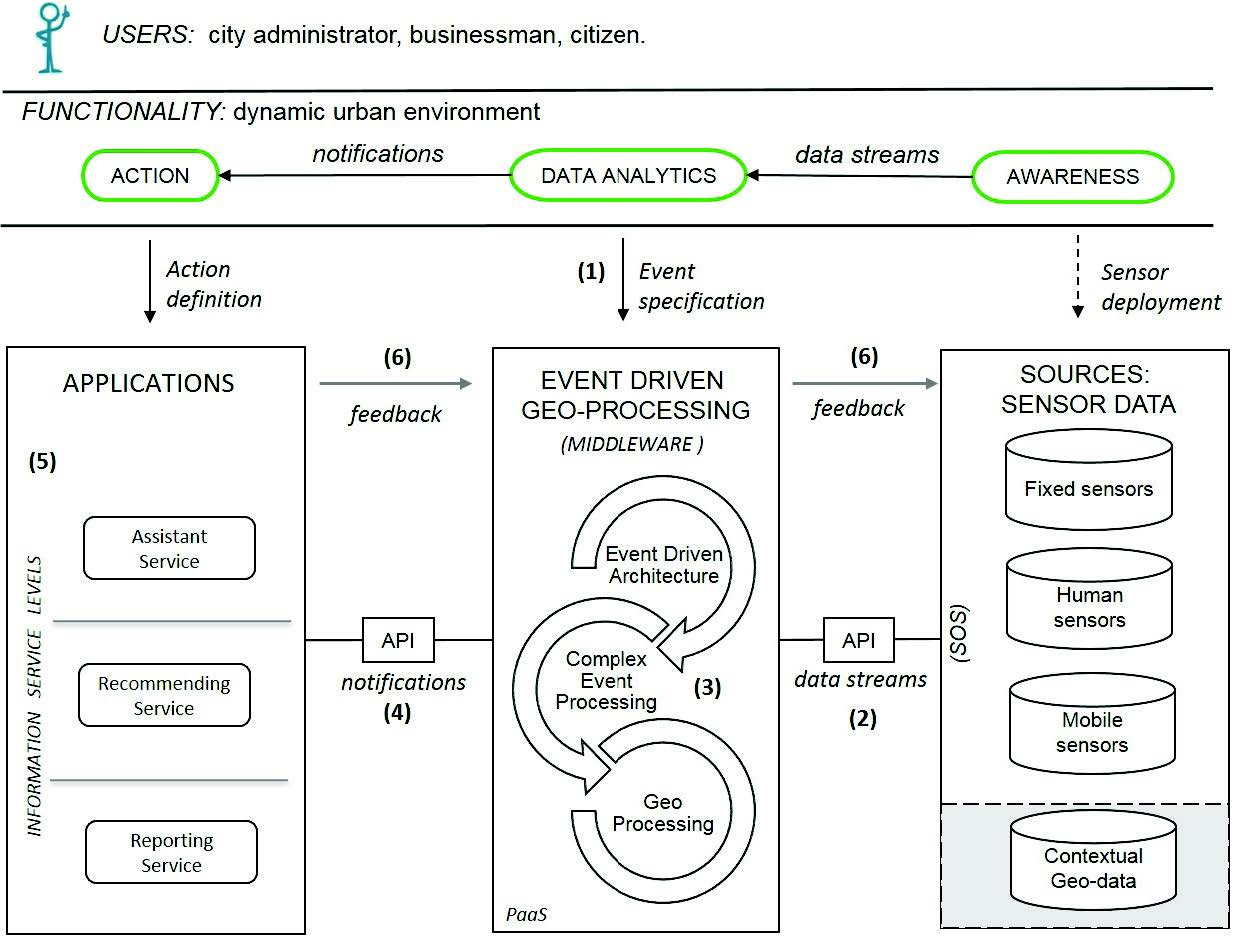
\includegraphics[width=\textwidth]{Morales_2015}
	\caption{Event-driven geoprocessing system architecture~\cite[p.~3]{Morales.2015}}
	\label{fig:morales-arch}
\end{figure}

\begin{figure}[h]
	\centering
	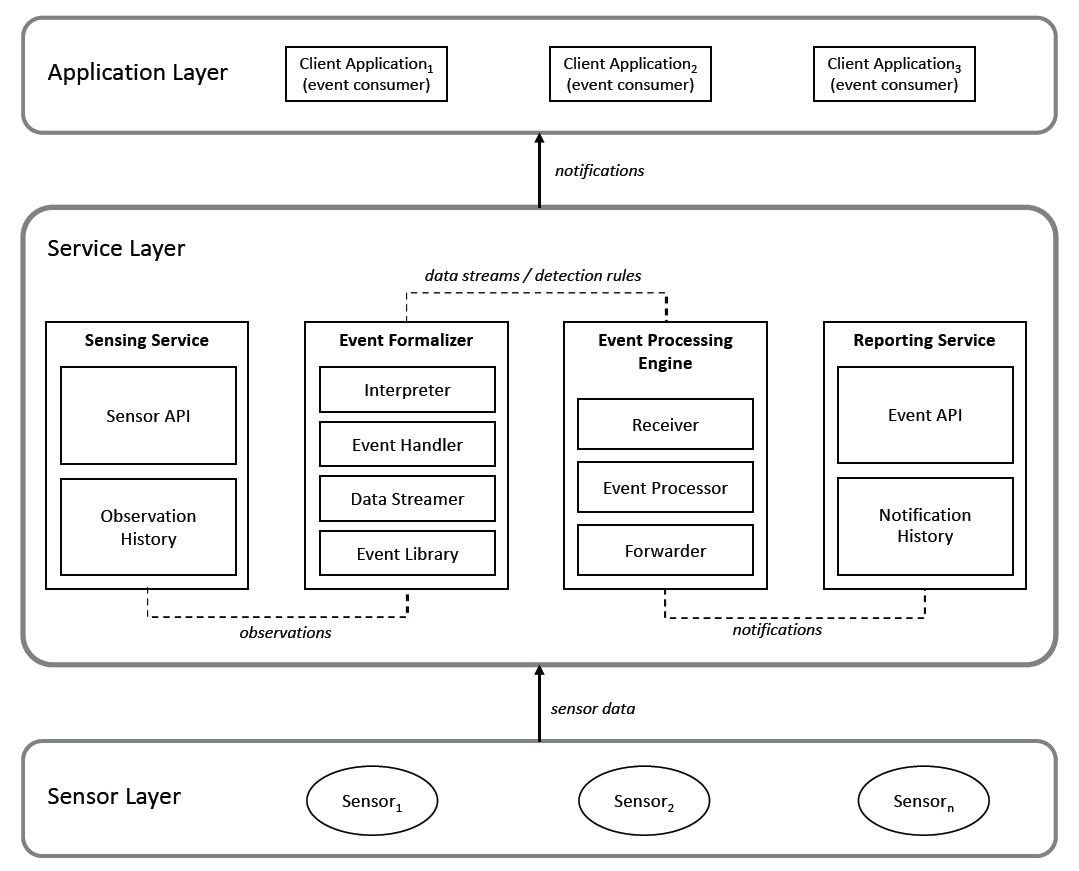
\includegraphics[width=\textwidth]{Garcia_2019a}
	\caption{Reference Architecture for Smart City Applications (RASCA)~\cite[p.~12]{GarciaAlvarez.2019}}
	\label{fig:rasca}
\end{figure}

\begin{figure}[h]
	\centering
	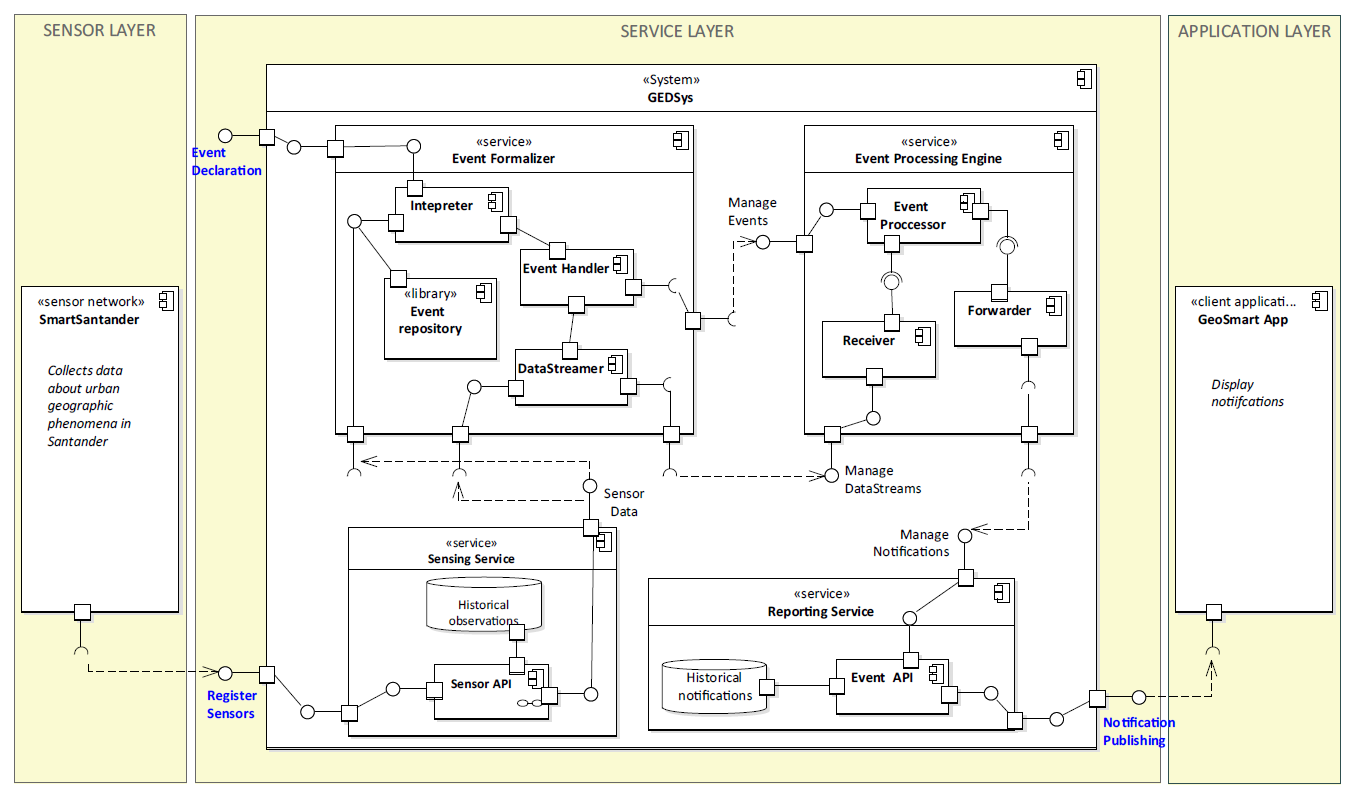
\includegraphics[width=\textwidth]{Garcia_2019b}
	\caption{Implementation of RASCA~\cite[p.~13]{GarciaAlvarez.2019}}
	\label{fig:rasca-impl}
\end{figure}

The architecture in Figures \ref{fig:rasca} and \ref{fig:rasca-impl} is an instantiation of Figure \ref{fig:morales-arch} and was used with data from SmartSantander project to detect geospatial events, e.g. temperature above \SI{0}{\celsius} in the city center. Mentions that Flink has good throughput but no geospatial matching capabilities. 

\begin{figure}[h]
	\centering
	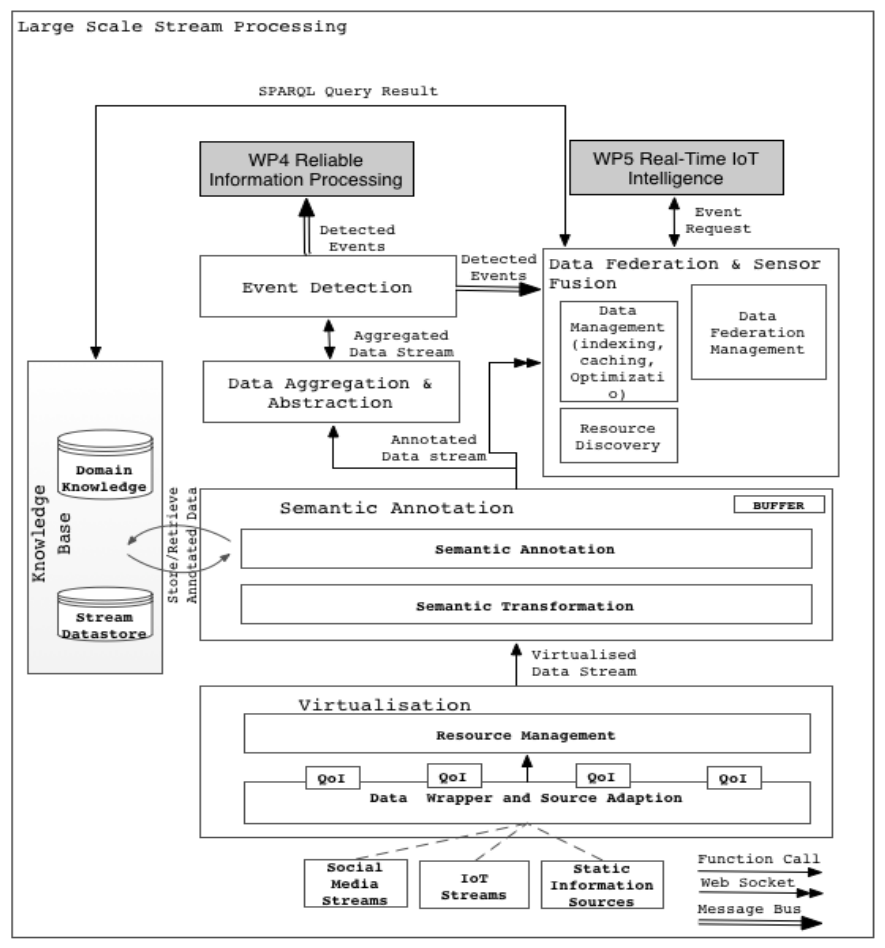
\includegraphics[width=\textwidth]{Tsiatsis_2015}
	\caption{Large Scale Data Analysis Functional Group for CityPulse~\cite[p.~25]{Tsiatsis.2015}}
	\label{fig:citypulse-streaming}
\end{figure}

The CityPulse project described in \cite{Tsiatsis.2015}, \cite{Presser.2016}, \cite{Puiu.2016} \cite{Puiu.2016b} uses AMQP for message transport. The stream processing is shown in Figure \ref{fig:citypulse-streaming}.

\section{Available Data}

\section{Visualization}

\section{Challenges}
\enquote{Geoprocessing of data streams inherits challenges from big data analysis: volume, velocity, variety, value, and veracity.}~\cite[p.~1]{Morales.2015}

\printbibliography


\end{document}
